% chapter 3 : teach-center
\chapter{Teach Center}

Inhalt.

\section{Schwarzes Brett}

\begin{figure}[htbp]
  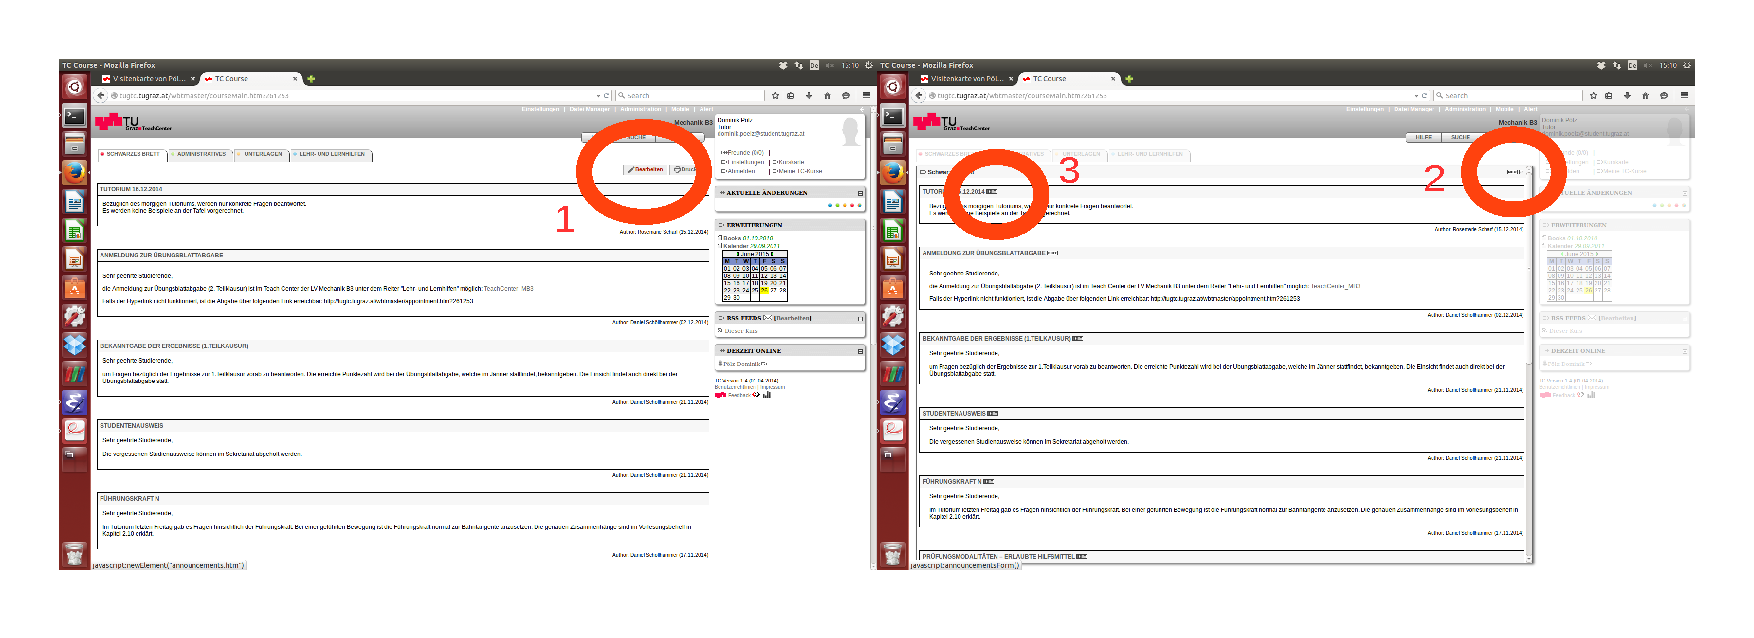
\includegraphics[width=\textwidth]{3_sb.pdf}
  \caption{ (1) Editieren des Schwarzen Brettes. (2) Erstellen eines neuen
    Beitrags. (3) Editieren eines bestehenden Beitrags.}
\end{figure}

\section{Lehr- und Lernhilfen}

\begin{figure}[htbp]
  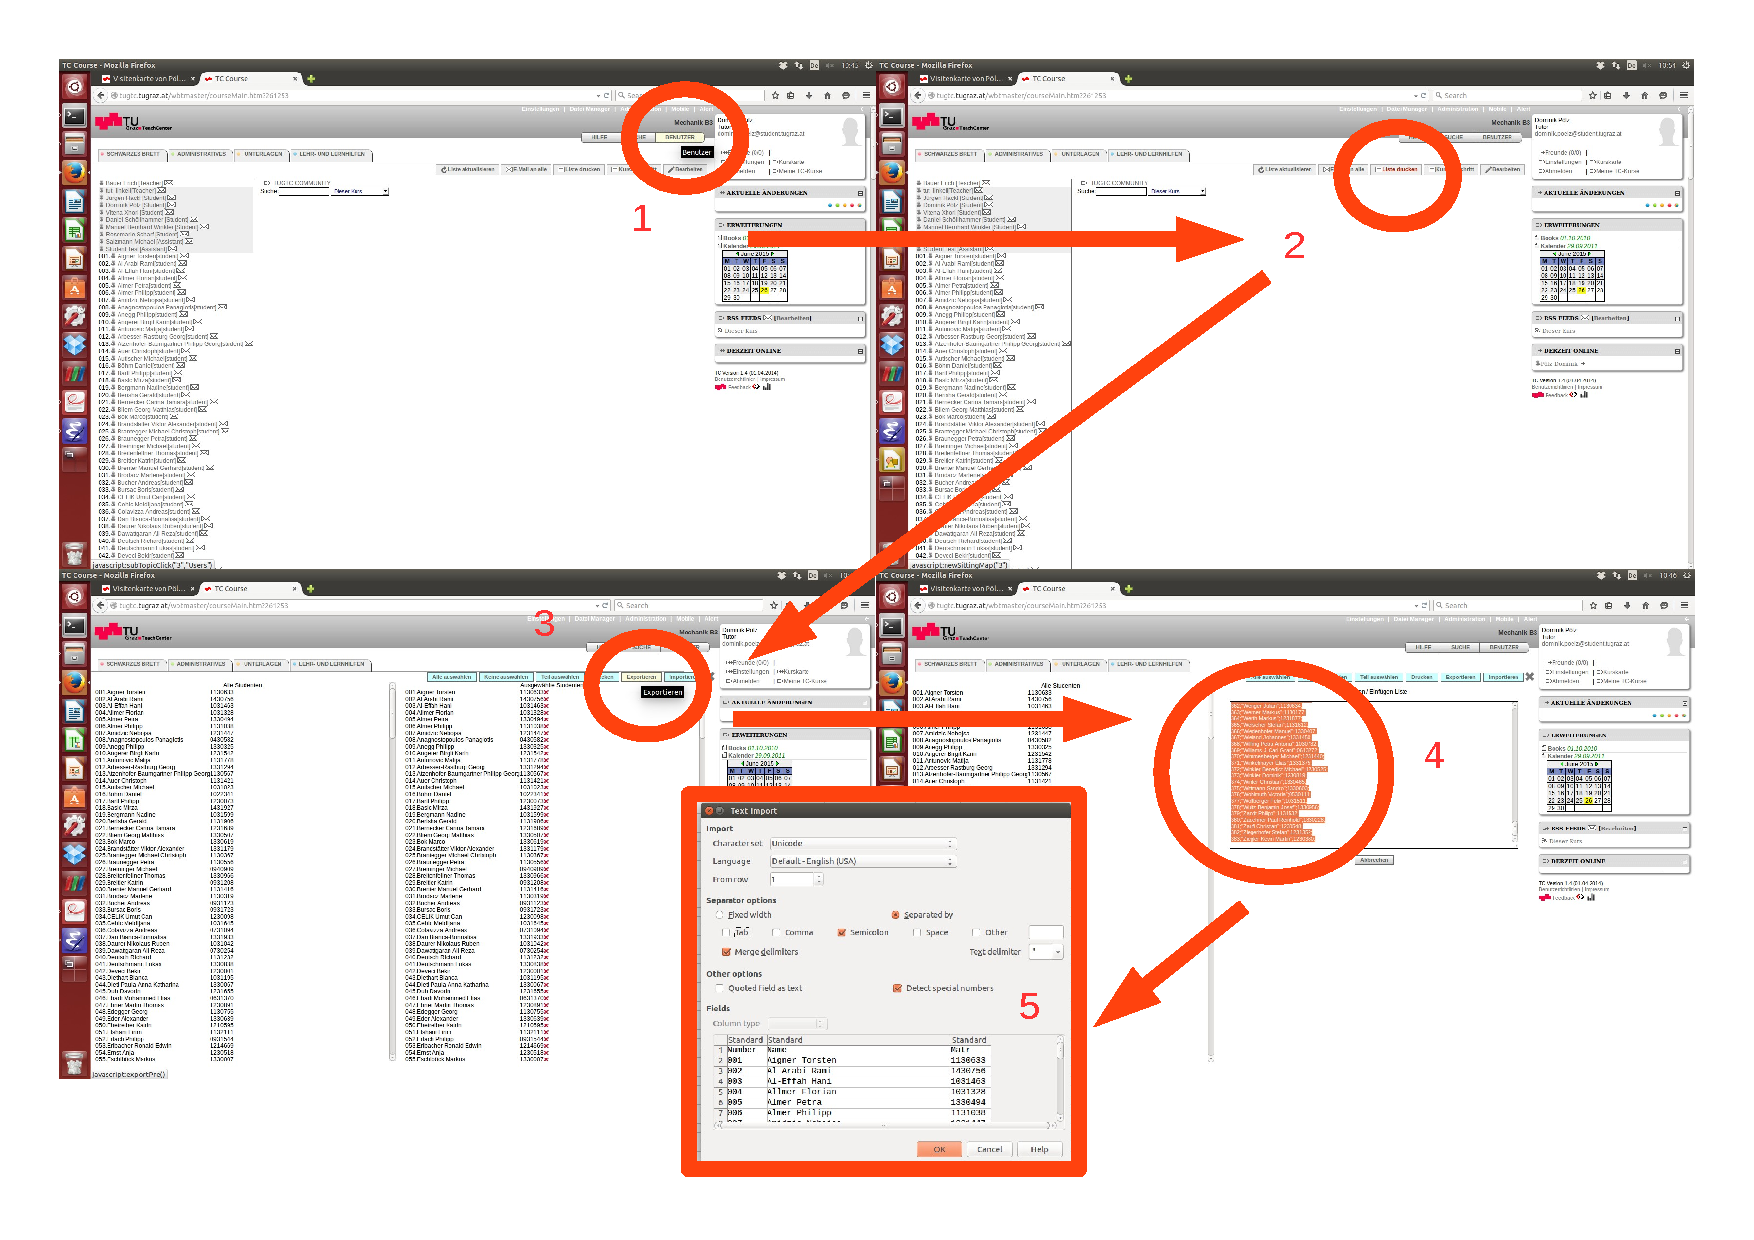
\includegraphics[width=\textwidth]{3_exportList.pdf}
  \caption{ (1) Auswahl Benutzer. (2) Liste drucken. (3) Alle ausw\"{a}hlen und
    exportieren. (4) Gesamten Inhalt kopieren und (5) in Excel einf\"{u}gen,
    wobei das richtige Trennsymbol zu w\"{a}hlen ist.}
\end{figure}

%EOF